\documentclass[a4wide,12pt]{report}
\usepackage[utf8]{inputenc}
\usepackage[IL2]{fontenc}
\usepackage{listings}
\usepackage{amssymb}
\usepackage{amsmath}
\usepackage{url}
\usepackage{graphicx}
\usepackage[czech]{babel}
%\usepackage{fullpage}
\usepackage[top=22mm, bottom=30mm, left=35mm, right=25mm]{geometry}
\usepackage{tikz}
\title{sds}
\author{Marek Bryša}
\date{Brno 2011}
\begin{document}
\tableofcontents

\chapter*{Úvod}
\addcontentsline{toc}{chapter}{Úvod}
\chapter{Prodejní síť Oriflame}
\section{Historie firmy Oriflame}
Firma Oriflame byla založena v roce 1967 ve Švédsku bratry Jonasem a Robertem Jochnick. Cílem bylo nabídnout lidem přirozenou a přírodní péči o svou pleť. Místo aby nákladně budovali kamenné obchody, rozhodli se dostat prodej přímo do domovů a využít tak vrozenou podnikavost lidí. Tento základní koncept zůstáva po více než 40 let nezměněn. V roce 1990, po po pádu železné opony, firma expanduje po střední a východní Evropě a zakládá pobočku i v České republice. V roce 2001 dosahuje počet kosmetických poradců jednoho miliónu a obrat téměř 450 miliónů EUR.

Sortiment je opravdu široký, katalog obsahuje přes 1500 výrobků v cenách přibližně od 50 do 1000 Kč. Většina typů produktů obsahuje několik cenou a kvalitou odlišených řad. Celkově lze říci, že zákazník má možnost nákupu komplexní péče s téměř libovolným rozpočtovým omezením.
\section{Podmínky síťového prodeje}
V této části popíšeme fungování sítě Oriflame na českém trhu. V jiných zemích se mohou zejména parametry mírně lišit. Prodejcem (v terminologii Oriflame \emph{poradcem}) se zájemce stane vyplněním jednoduchého formuláře a zaplacením poplatku 99 Kč. Tím získá možnost výdělku následujícími způsoby:
\begin{enumerate}
\item Nákupem kosmetických výrobků v centrech Oriflame nebo na objednávkou přes internet za tzv. nákupní ceny, které jsou o 30\% nižší než prodejní (katalogové) ceny. Prodejce tak realizuje 30\% marži z prodeje sobě a svým zákazníkům (typicky rodině a známým).
\item Plnou hodnotu tzv. \emph{slevy z obratu} svého vlastního prodeje.
\item Budováním skupiny poradců, které k Oriflame přivedl, tzv. \emph{sponzoroval}. Pak mu náleží rozdíl mezi svou slevou z obratu a slevou z obratu lidí, které k Oriflame přivedl a jejich skupin.
\end{enumerate}
Tento systém slouží jako motivace lidí pro rozšíření prodejní sítě. Je založen na očekávaní vysokého výdělku v budoucnosti. Firma ve svých materiálech jako příklad uvádí lineární růst výdělku pro poradce z prodeje a exponenciální ze sponzorování.

Rok je rovnoměrně rozdělen na 17 období, které odpovídají vydáním katalogů výrobků. Poradce, který podal v předchozích třech obdobích alespoň jednu objednávku, obdrží sadu tiskovin zdarma, jinak je pro něj téměř nutnost si tištěný katalog zakoupit za TODO:cena katalogu.

Firma dále nabízí pro začínající poradce ve čtyřech krocích motivaci ve formě věcných darů za splnění určitých objemů obratu, např. v prvním kroku za obrat 1250 Kč tašku, průvodce péčí o pleť a krém v celkové hodnotě 510 Kč.

Také jsou k dispozici úvěry do výše 7000 Kč na zaplacení za zobží, které hodlá poradce dodat zákazníkum a nemusí tak od nich vybírat peníze předem.

Oriflame poskytuje garanci vrácení peněz do 30 dnů od nákupu výrobku bez udání důvodu a to i v případě, že výrobek obsahuje minimálně 80\% původního objemu.
\subsection{Skupiny a slevy z obratu}
Každému výrobku jsou v ceníku přiděleny čtyři hodnoty:
\begin{description}
\item[PC] Doporučená prodejní cena spotřebitelům.
\item[NC] Nákupní cena včetně DPH. Za tu poradci mohou zobží zakoupit v centrech Oriflame.
\item[OO] Obchodní obrat. Typicky je roven nákupní ceně bez DPH. V případě nespotřebních produktů (např. kartáč na vlasy, houba na mytí) je ještě přibližně poloviční.
\item[BO] Bodové ohodnocení. Na inflaci nezávislý počet bodů, které poradce nákupem zboží získá. V současnoti odpovídá přibližně 13,80 Kč obchodního obratu.
\end{description}
Výjimku tvoří např. tiskoviny, vzorky a oblečení s logem Oriflame, které mají pouze nákupní cenu,  nejsou určeny k dalšímu prodeji a slouží jen jako pomůcka pro poradce.

Poradce dále získá body všech lidí které přivedl a těch pod nimi. Na konci každého katalogového období dochází k vyhodnocení. Sečtou se všechny body a podle následujícího klíče se určí procentní úroveň:
\begin{center}
\begin{tabular}{|l|c|c|c|c|c|c|c|}
\hline
body & $\geq$200 & $\geq$600 & $\geq$1200 & $\geq$2400 & $\geq$4000 & $\geq$6600& $\geq$10000\\\hline
úroveň & 3\% & 6\% & 9\% & 12\% & 15\% & 18\% & 21\%\\\hline
\end{tabular}
\end{center}
Toto se provede i pro všechny podskupiny. Poradce pak získá za každou podskupinu: obchodní obrat skupiny $\cdot$ (procentní úroveň poradce $-$ procentní úroveň skupiny). Tím je zajištěno, že člověk, který se stal poradcem Oriflame později, ale je schopnější, může dosáhnout vyššího výdělku než ten, kdo jej přivedl. Poradce také obdrží přímo podle své procetní úrovně slevu ze svého vlastního prodeje.

Všechny tyto peníze poradce dostane na účet. Podmínkou je, že jeho vlastní prodej musí dosáhnout 100 bodů. To firma zdůvodňuje tím, že poradce musí být sám schopným prodejcem, aby mohl učit ostatní.

Při dosažení 12\% úrovně se poradce stává tzv. manažerem, při 21\% direktorem. Za to má možnost získat věcné i finanční prémie, účast na školeních aj. V případě, že osoba na 21\% úrovní sponzoruje někoho, kdo jí dosáhl také, stanovuje se procetní rozdíl úrovní na 3\%.
\\TODO: priklad grafu skupiny?
\\\tikz
\node {Computational Complexity\\dsa} % root
child { node {Computational Problems}
child { node {Problem Measures} }
child { node {Problem Aspects} }
child { node {Problem Domains} }
child { node {Key Problems} }
}
child { node {Computational Models}
child { node {Turing Machines} }
child { node {Random-Access Machines} }
child { node {Circuits} }
child { node {Binary Decision Diagrams} }
child { node {Oracle Machines} }
child { node {Programming in Logic} }
}
child { node {Measuring Complexity}
child { node {Complexity Measures} }
child { node {Classifying Complexity} }
child { node {Comparing Complexity} }
child { node {Describing Complexity} }
}
child { node {Solving Problems}
child { node {Exact Algorithms} }
child { node {Randomization} }
child { node {Fixed-Parameter Algorithms} }
child { node {Parallel Computation} }
child { node {Partial Solutions} }
child { node {Approximation} }
};

\chapter{Popis modelu}
V této kapitole se budeme věnovat popisu modelu sítě Oriflame z technického a ekonomického pohledu. Dojde i k částečnému prolnutí se implementací modelu na počítači, což je nutné, aby si jej čtenář mohl v případě potřeby snáze upravit.
\section{Technický popis}
Pro vytvoření experimentálního modelu bylo zvoleno prostředí NetLogo ve verzi 4.1.3. Je to oteřený a volně šiřitelný software umožňující snadnou tvorbu agentových a systémově-dynamických modelů. Běh modelu zahrnuje zpravidla dvě části:
\begin{enumerate}
\item Inicializace (setup). Zde se nastaví všechny proměnné na výchozí hodnoty, většinou také dojde k vygenerování náhodných parametrů a vztahů pro jednotlivé agenty.
\item Vlastní běh. Ten probíhá v opakovaných oddělených krocích. V každém z nich dojde k projevu chování agentů a tím změně promenných, vztahů mezi agenty atd.
\end{enumerate}
V tomto modelu se pracuje zejména s agenty \texttt{person}, obousměrným vztahem \texttt{friend} a jednosměrným \texttt{sponsor}.
\section{Ekonomický popis}
\subsection{Generování sociálních vazeb}
Je nutné, aby model věrně zachytil sociální vztahy ve společnosti. Každý agent ma jistý okruh přátel, kterým může prodávat kosmetické výrobky a nabídnout jim členství v prodejní síti. Model obsahuje konstanty \texttt{number-of-persons} a \texttt{number-of-friendships}. První značí počet vygenerovaných osob, druhá počet náhodných přátelství mezi nimi. Je nutné aby graf tovřil jednu komponentu, protože na světě prakticky neexistují uzavřené a s nikým nekomunikující skupiny lidí. To je zajištěno tak, že ihned po vygenerování všech lidí každý postupně vytvoří přátelství s někým, kdo už nějaké má. Tím vzniká mírné vychýlení oproti jinak normálnímu rozdělení počtu přátelství na osobu, které je ale vzhledem k počtu dále přidaných přátelství zanedbatelné. Na následujících dvou grafech jsou histogramy jednoho běhu generování přátelství pro \texttt{number-of-persons}=\texttt{number-of-friendships}=300 před a po přidání náhodných přátelství:\\
\begin{center}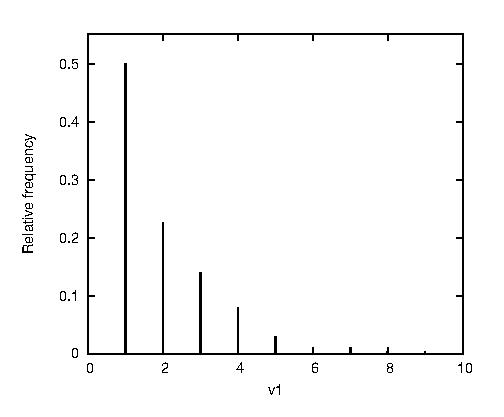
\includegraphics{hist_fr_v1.eps}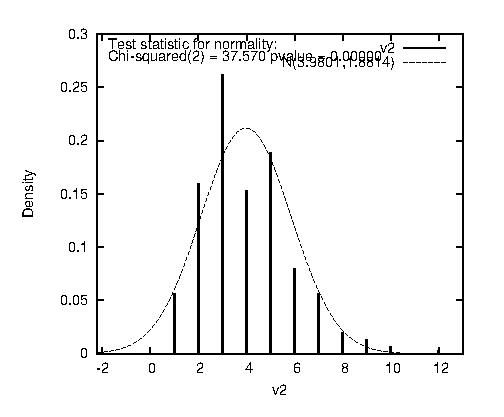
\includegraphics{hist_fr_v2.eps}\end{center}
\subsection{Prostředí}
Agenti jsou generování v izolovaném prostředí. Na začátku je jeden z nich určen jako zdrojový a od něj se pak síť může postupně po jednotlivých kolech šířit. Je možne také zapnout volbu \texttt{random-join?}, která znamená, že v každém kole je nabídnuto členství jednomu náhodnému agentovi --- nečlenovi. To modeluje případ, kdy se poradci snaží o nábor lidí např. u stánků.

Dále jsou přítomny tyto za běhu měnitelné konstanty:
\begin{description}
\item[\texttt{margin}] Marže pro prodejce.
\item[\texttt{monthly-fee}] Poplatek za členství placený v každém kole. Firma Oriflame jej nevybírá, je tedy určen spíše pro experimenty.
\end{description}
\subsection{Vlastnosti agenta \texttt{person}}
Agent \texttt{person} představuje v modelu jednoho člověka. Má tyto důležité vlastnosti:
\begin{description}
\item[\texttt{consupmtion}] Množství peněz, které daná osoba během jednom období může utratit za kosmetické výrobky, které je možno koupit v síti Oriflame. Je to ekvivalent rozpočtového omezení a považuje se za konstantní. Ve výchozím nastavení je generováno jako:
$$\max\{100,\texttt{random-normal(1000,500)}\}$$
Tj. náhodná hodnota z normálního rozdělení se střední hodnotou 1000, rozptylem 500, zdola omezená 100 (spořeba nižší než 100 by byla nevýznamná).
\item[\texttt{netmember?}] Značí, zda je agent členem sítě --- poradcem.
\item[\texttt{be-point}] Bod ukončení činnosti. Členstvím v síti vznikají každému náklady. Tvoří je explicitní např. výdaje za cestu k zakazníkům a implicitní za čas obětovaný této práci. Obecně lze říci, že implicitní složka bude tím vyšší, čím lépe na daný člověk placené hlavní zaměstnání. A tím se také zvyšuje jeho rozpočtové omezení. Proto existuje závislost mezi consumption a be-point vyjádřená:
$$\max\{\texttt{consumption}\cdot 0.5,\texttt{consumption}\cdot\texttt{random-normal(1,0.5)}\}$$
\end{description}
\subsection{Chování agenta \texttt{person}}
Chování vychází z jednoduché racionálni úvahy --- vyplatí se do sítě vstoupit a zůstat v ní? Lze jej tedy rozdělit na dvě části: podmínku vstupní a podmínku setrvání.
\subsubsection{Vstupní podmínka}
Pokud je agentovi nabídnuto členství, přijme ho pokud:
$$(\texttt{myrev} + \texttt{avg-exp-rev}) \cdot (1+\texttt{d-margin}) \geq \texttt{be-point} + \texttt{monthly-fee}$$
kde:
\begin{description}
\item[\texttt{myrev}] je očekávaný příjem z přímeho prodeje přátelům agenta. Vypočítá se jako: $$\sum_{p\in F}(\texttt{consumption}_p\cdot\texttt{margin})$$
kde $F$ je množina přátel. Pokud některému z nich může zboží dodávat více poradců, je spotřeba rozdělena rovnoměrně mezi ně.
\item[\texttt{avg-exp-rev}] je očekávaný příjem ze sponzoringu a skupin. Protože v rozhodování člověka je jistá setrvačnost, je dán jako průměr posledních deseti skutečných příjmů z této činnosti. Při inicializaci je naplněn těmito hodnotami:
\[ 0.09\cdot (\sum_{p\in F}\texttt{consumption}_p)\cdot |F|^{1.3} \]
To odpovídá odhadu uváděnému při nabídce členství v síti.
\item[\texttt{d-margin}] je rozdíl mezi současnou \texttt{margin} a tou při posledním odchodu agenta ze sítě, nejméně 0. To proto, že pokud se marže od posledního pokusu o nábor člena zvýšila, bude to použito jako argument, v opačném případě spíše zamlčeno.
\end{description}
\subsubsection{Podmínka setrvání}
Ta je dána velmi podobně:
\[ \texttt{avg-exp-rev} + \texttt{my-rev} \geq \texttt{be-point} + \texttt{monthly-fee} \]
\texttt{my-rev} v tomto případě již není odhad, ale skutečná hodnota.
\chapter{Experimenty}
\begin{thebibliography}{9}

\bibitem{fd}

\end{thebibliography}
\url{http://www.oriflame.com/About_Oriflame/History/}
cenik 4/2011
manual kosmetickeho poradce
http://ccl.northwestern.edu/netlogo/download.shtml
\end{document}

